\documentclass[12pt, a4paper, twoside]{article}

\usepackage{fontspec}
\usepackage{blindtext}
\usepackage{geometry}
\usepackage{setspace}
\usepackage{titlesec}
\usepackage{indentfirst}
\usepackage{graphicx}
\usepackage[italian]{babel}

% FIXME swap to calibri on windows? no license for linux
\setmainfont{Carlito}
\titlespacing*{\section}{0px}{3mm}{1mm}
\titlespacing*{\subsection}{0px}{3mm}{1mm}
\geometry{
  left=2cm,
  right=2cm,
  top=2cm,
  bottom=2cm
}
\setlength{\parindent}{10mm}
\graphicspath{ {./assets} }

\begin{document}

\begin{center}
  \huge Titolo \\
  \large Francesco Platini 000000000000. Matteo Bonacini 0000000000.\\
  Data
\end{center}

% Title spacing

\section{Abstract}\label{sec:abstract}
  In questo esperimento abbiamo analizzato il comportamento di un raggio di luce
  che colpisce la superficie di un prisma di materiale ignoto.
  Abbiamo verificato che l’intensità luminosa riflessa segue l’andamento
  previsto dalle leggi di Fresnel e abbiamo misurato l’angolo di Brewster per il
  materiale del nostro prisma.
  I risultati ottenuti sono ?????????? compatibili/incompatibili

\section{Introduzione}\label{sec:introduzione}
  Quando un raggio luminoso colpisce una superficie di separazione tra due mezzi
  dielettrici con indici di rifrazione $n_1$ e $n_2$ diversi, si possono verificare
  i fenomeni della riflessione e rifrazione della luce.
  Le equazioni di Fresnel, derivabili direttamente dalle Equazioni di Maxwell,
  descrivono questo comportamento prevedendo quale frazione d'intensità
  luminosa viene riflessa e rifratta, per ciascuna delle due componenti di
  polarizzazione.
  Indichiamo con $R_\pi$ e $R_\sigma$ le frazioni d'intensità luminosa riflessa
  polarizzata, rispettivamente, parallelamente e perpendicolarmente al piano
  d'incidenza.
  Si dimostra che valgono:

  \begin{equation}
    R_\pi = \frac {
      n_2 \cos{\theta_i} - n_1 \cos{\theta_t}
    } {
      n_2” \cos{\theta_i} + n_1 \cos{\theta_t}
    }\label{eq:fresnel equation 1}
  \end{equation}

  \begin{equation}
    R_\sigma = \frac {
      n_1 \cos{\theta_i} - n_2 \cos{\theta_t}
    } {
      n_1” \cos{\theta_i} + n_2 \cos{\theta_t}
    }\label{eq:fresnel equation 2}
  \end{equation}

  \noindent dove $n_1$ e $n_2$ sono gli indici di rifrazione dei due mezzi, $\theta_i$ e
  $\theta_r$ sono gli angoli d'incidenza e rifrazione del raggio luminoso.
  Una dimostrazione rigorosa di come si ricavino queste equazioni non è oggetto
  di questo testo, ma si rimanda a Mazzoldi[1] per ulteriori approfondimenti. % todo add reference
  Variando l’angolo d'incidenza e misurando l’intensità in funzione di tale, si
  può vedere l’andamento dei due coefficienti.
  Le formule prevedono che $R_\pi$ si annulli per un certo valore di $\theta_i$,
  che indicheremo con $\theta_B$.
  Questo angolo prende il nome di Angolo di Brewster, ed è dato dalla Legge di Brewster:

  \begin{equation}
    \theta_B = \arctan{
      \frac {n_2} {n_1}
    }\label{eq:Brewster's law}
  \end{equation}

 \noindent  L’angolo di Brewster gode di alcune proprietà utili in diverse applicazioni
  sperimentali.
  Per approfondimenti, rimandiamo a [Mazzoldi].



\section{Apparato sperimentale e svolgimento}\label{sec:apparato-sperimentale-e-svolgimento}
  \subsection{Apparato sperimentale}\label{subsec:apparato-sperimentale}
    L’apparato sperimentale, riportato in [fig.1] è formato da un prisma
    posizionato al centro di una guida circolare graduata. Il prisma è montato
    ad un servomotore (??? modello) che gli permette di ruotare con una
    risoluzione angolare di 1.0° +/- 0.5°. (todo: il goniometro ha permesso di
    misurare l’angolo iniziale da cui far partire l’acquisizione). Un laser è
    puntato verso il cristallo, e due filtri polarizzatori sono posti in mezzo
    al fascio. Alla guida rotante è collegato un sensore di intensità luminosa
    (??? Modello).
    Il servo ed il sensore sono collegati a (?? mettere davvero tutto il setup
    oppure solamente una roba) una scheda arduino, che si occupa dell’acquisizione
    dei dati.
    (todo inserisci numeri della roba)

    Todo add specifiche di tutta la roba e link to datasheet.
    ADC arduino, reference voltage e cazzate varie
    Considerazioni su come l’errore sul sensore sia determinato principalmente da difficoltà nell’allineamento e da fluttuazioni del laser.

    \begin{figure}[h]
      \centering
      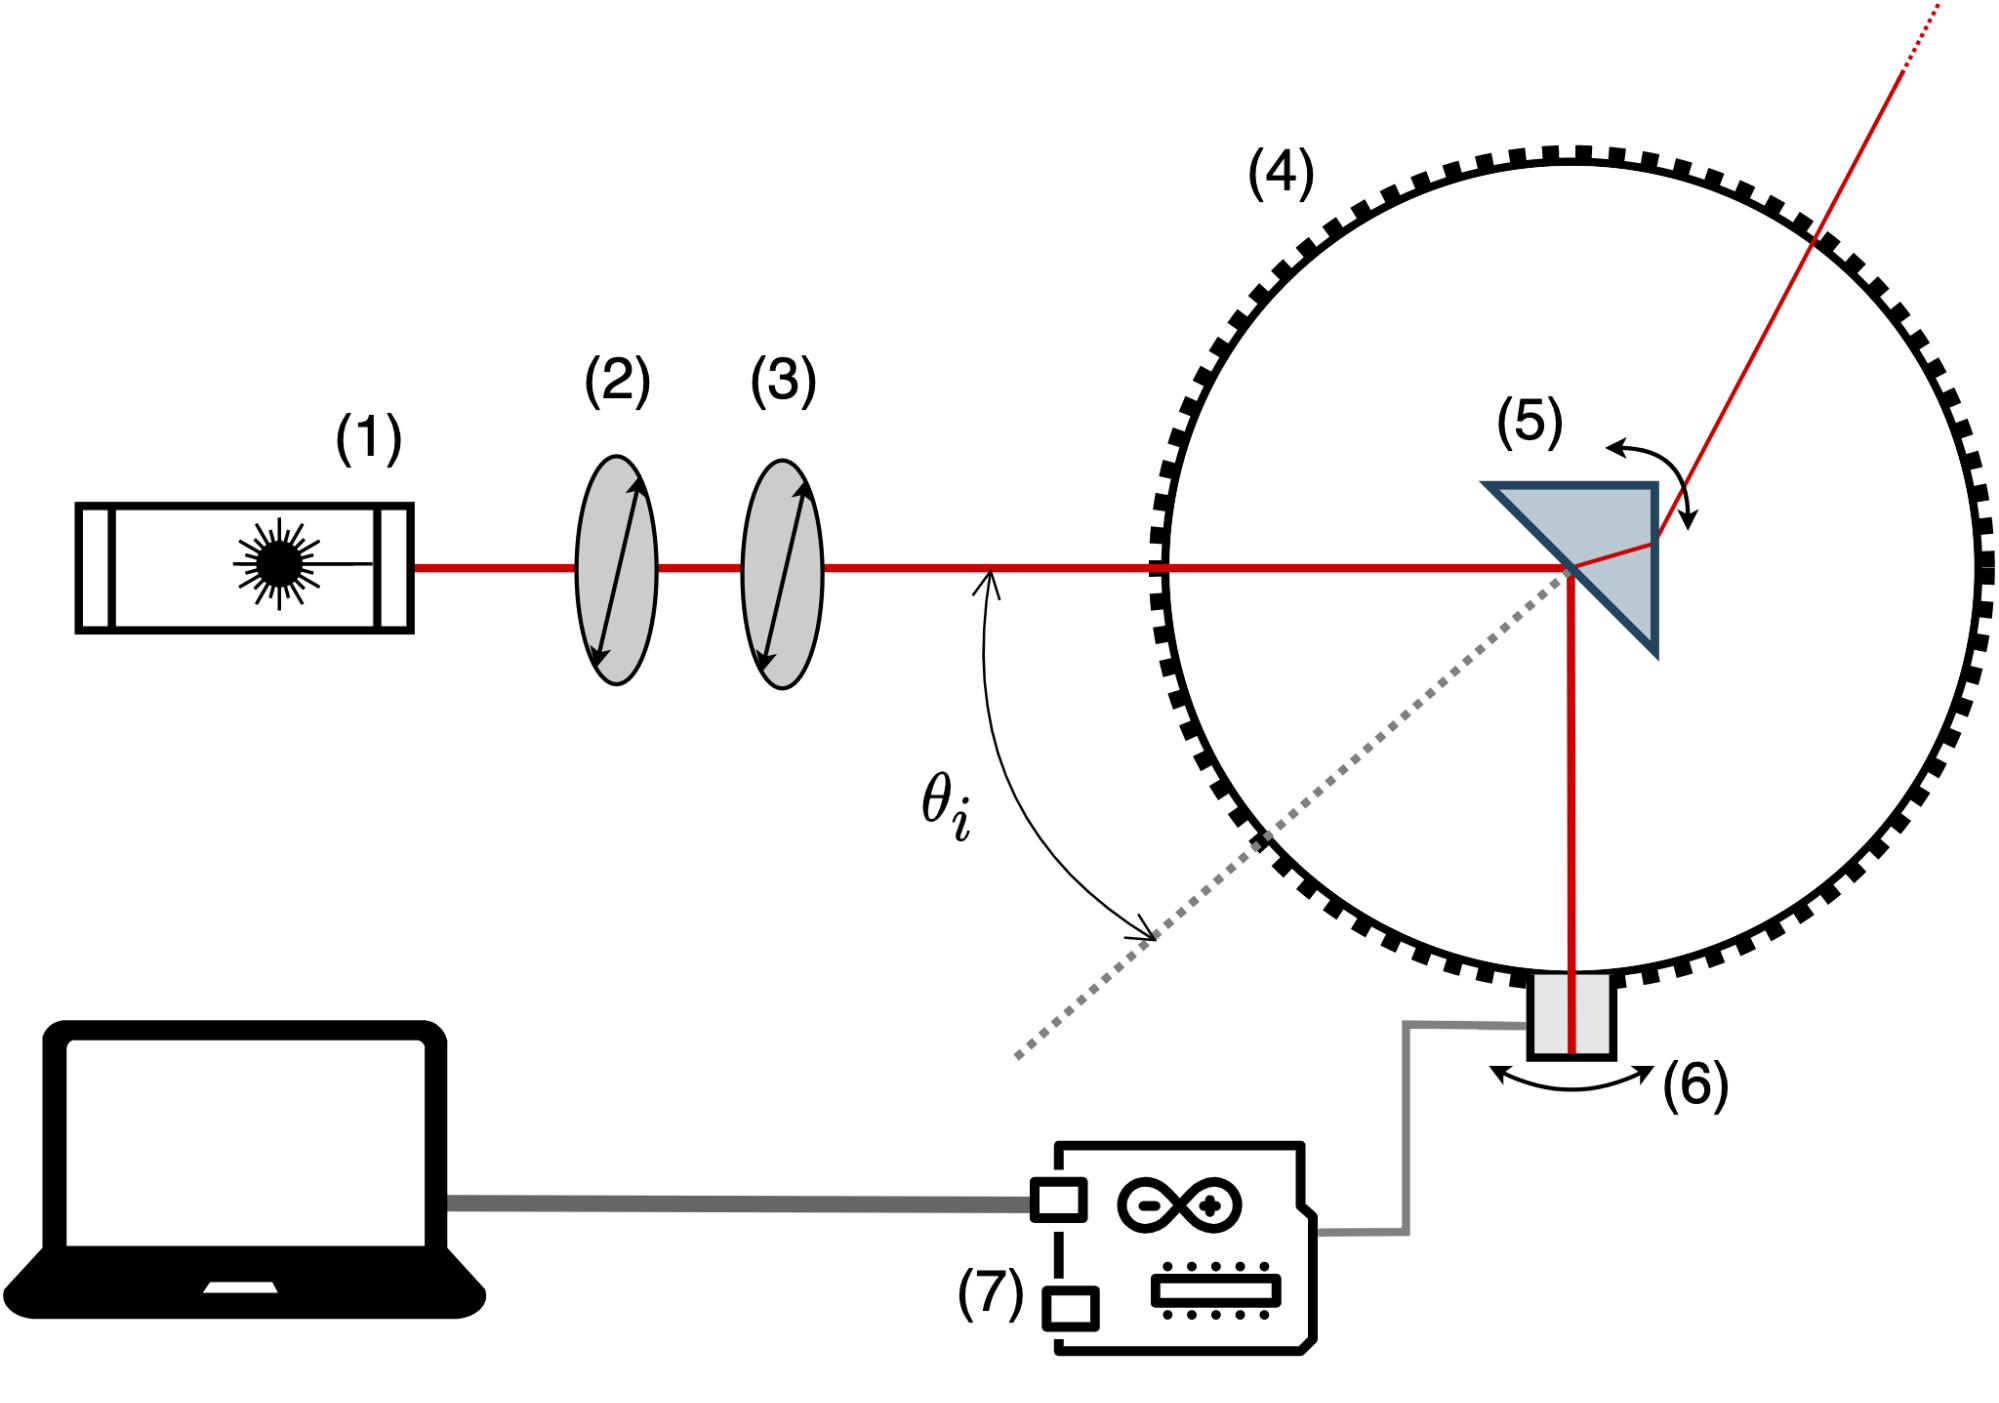
\includegraphics[width=10cm]{instrumental-apparatus.png}
      \caption{
        \emph{
          Apparato sperimentale. A partire da sinistra, in senso orario,
          si trovano: laser(1), filtri polaroid(2, 3), guida circolare(4),
          prisma(5), sensore(6), Arduino(7).
        }
      }
      \label{fig:instrumental-apparatus}
    \end{figure}

  \subsection{Procedura sperimentale}\label{subsec:procedura-sperimentale}
    Abbiamo iniziato misurando l’andamento del coefficiente $R_\pi$. Partiamo posizionando il secondo polaroid in modo che la polarizzazione della luce sia parallela al lato del prisma. Il laser che abbiamo utilizzato emetteva luce polarizzata, quindi abbiamo dovuto aggiustare anche il suo angolo rispetto al polaroid. Prima di iniziare le misure, abbiamo regolato l’intensità del laser in modo che il sensore potesse rilevare un range di valori il più ampio possibile. Abbiamo quindi posizionato il sensore direttamente davanti al laser e abbiamo ruotato il primo filtro polaroid, fino a che il sensore non è riuscito a rilevare una variazione significativa di intensità.
    Per prendere le misure, abbiamo iniziato ruotando il prisma in modo da massimizzare $\theta_i$. Per raccogliere un
    punto dati abbiamo allineato il sensore con il fascio laser riflesso e ne abbiamo misurato l’intensità. Abbiamo
    ripetuto questa misura riducendo man mano il valore di $\theta_i$, fino ad arrivare il più vicino possibile a $0\deg$.
    Il nostro apparato sperimentale ci ha permesso di svolgere misure per ?? < $\theta_i$ < ??.
    Abbiamo poi ruotato il secondo polaroid di 90° e ripetuta la stessa procedura per misurare $R_\sigma$.
    In questo modo, abbiamo ottenuto le misure di intensità riflessa $I_\pi$ e $I_\sigma$ [fig ??]. Per ottenere i
    coefficienti di Fresnel, abbiamo normalizzato i dati ottenuti tenendo conto che:
    there is no difference between Rp and Rs at normal incidence
    at glancing angle in the less-dense medium the reflection coefficients are ±1,
    Come descritto in [Lipson]
    Da queste misure abbiamo ricavato anche l’angolo di Brewster, osservando per quale valore di $\theta_i$
    l’intensità $I_\pi$ si annulla.


\section{Risultati e discussione}\label{sec:risultati-e-discussione}
  \blindtext[2]

\section{Conclusioni}\label{sec:conclusioni}
  \blindtext[1]

\newpage
\section{Appendice}
  \subsection{Calcolo incertezza strumentale}
    La fonte principale di incertezza strumentale è dovuta alla precisione dell’ADC del microcontrollore, e dalla precisione del potenziale di riferimento della scheda.
    L’incertezza strumentale del sensore è considerata trascurabile, e qualsiasi suo effetto sarà incluso nelle incertezze casuali che abbiamo considerato.

    L’incertezza dell’ADC è stata ottenuta direttamente dal datasheet della scheda ATmega328P (sezione 23.1 ADC
  Features). L’incertezza assoluta indicata dal costruttore della scheda è di $$\pm$$ 2LSB(todo spiega LSB). Questo
  valore tiene conto di tutte le possibili fonti di errore interne all’ADC, ed è un limite conservativo per l’errore.

    Per effettuare le misure, l’ADC utilizza il segnale “VREF(1.1V)” della scheda arduino come segnale di
calibrazione. L’incertezza di VREF è stata stimata da (riferimento), e ha come limite superiore lo 0.4\%. La formula
che utilizziamo per ottenere il valore (espresso in LSB) del segnale in entrata è:
    % I_{cor} = \frac {
    %   V_{ref} * 1000 * I_{raw}
    % } {
    %   V_{cc} V_{max}
    % }
    Dove $I_{corr}$ è il segnale corretto tramite $V_ref, I_{raw}$ è il segnale letto dall’ADC prima di apportare la correzione, $V_{max}$ è il potenziale massimo reale che vogliamo misurare.
    Propagando l’incertezza su $V_{ref}$ si ottiene quindi che $I_{corr}$ ha un incertezza associata di 0.4%.
    L’errore iniziale di offset di VREF è stato ignorato, visto che per le nostre misure si traduce solamente in un fattore moltiplicativo (a noi non interessa un valore assoluto di intensità, ma l’importante è i dati misurati siano tutti in proporzione).

    L’incertezza strumentale totale è quindi di $\pm$ 2LSB $\pm$ 0.4%

  \subsection{Calcolo errore 2}
    A causa di limitazioni strumentali, non ci è stato possibile ottenere un campione
    significativo di misure di intensità per ogni angolo. Possiamo comunque ottenere
    una stima delle incertezze casuali facendo una semplice assunzione: osserviamo che
    tra un angolo e un altro, il nostro apparato sperimentale non cambia; di conseguenza,
    se potessimo prendere un numero molto grande di misure per ogni valore di theta,
    ci aspetteremmo di ottenere una serie di distribuzioni di intensità $I_\theta$
che differiscono solo per il valore medio, ma non per la deviazione standard.
Per stimare questa deviazione standard, quindi, abbiamo calcolato la semmidispersione
massima (miglior stima di deviazione standard per poche misure) per tutte le serie
di misure fatte sullo stesso angolo, e come sigma abbiamo preso la media di queste.

\end{document}

%In this document somasdmeters
%were added. There is an encoding package,
%and pagesize and fontsize parameters.
